\documentclass[letterpaper, 10 pt, conference]{IEEEtran}
\IEEEoverridecommandlockouts
\overrideIEEEmargins

% --- Packages ---
\usepackage{cite}
\usepackage{amsmath,amssymb,amsfonts}
\usepackage{algorithmic}
\usepackage{graphicx}
\usepackage{textcomp}
\usepackage{xcolor}
\usepackage{booktabs}
\usepackage{multirow}
\usepackage{hyperref}

\newtheorem{theorem}{Theorem}
\newtheorem{lemma}{Lemma}
\newtheorem{definition}{Definition}

\begin{document}

\title{\LARGE \bf
The Topological Cage: Search-Less Geometric Injection and \\ Adaptive Spring-Mass Routing for Multi-Query Navigation
}

\author{Shubham Puri Goswami$^{1}$ and Ravi Prakash$^{2}$% <-this % stops a space
\thanks{$^{1}$Shubham Puri Goswami is with Cyber Physical Systems, Indian Institute of Science, Bengaluru, India {\tt\small shubhampg@iisc.ac.in}}%
\thanks{$^{2}$Ravi Prakash is with Cyber Physical Systems, Indian Institute of Science, Bengaluru, India {\tt\small ravipr@iisc.ac.in}}%
}

\maketitle
\thispagestyle{empty}
\pagestyle{empty}

% ==========================================
% ABSTRACT
% ==========================================
\begin{abstract}
Traditional sampling and grid-search algorithms scale poorly in large environments and frequently yield trajectories that hazardously graze obstacle boundaries. While skeletonization methods, such as the Medial Axis Transform, offer provably high-clearance topological backbones, their real-world deployment is severely bottlenecked by two critical flaws. First is the ``Injection Problem'': the inability to safely route an off-road robot onto the skeletal graph without reverting to exhaustive local search. Second is the ``Voronoi Void'': the tendency of traditional equidistance-based Voronoi algorithms to generate sparse, disconnected branches in expansive open spaces, stranding the robot. 

We propose the \textit{Topological Cage}, a strictly geometric framework that resolves these vulnerabilities by modeling free space as a continuous scalar field. By algorithmically bounding the medial axis into a closed topological manifold, our method unites all disconnected components and isolated islands during a one-time offline compute. For online routing, bi-directional gradient scouts guarantee start-to-goal injection in $\mathcal{O}(1)$ grid expansions, decoupling map processing from route generation. This extreme computational efficiency enables exhaustive real-time sampling of all available topological paths. To resolve homotopy degeneracy, we introduce a lexicographical bottleneck evaluator, smoothing the final optimal trajectory via selective obstacle-bound trimming and a distributed spring-mass elastic band. Validated on a differential-drive robot utilizing a motion-capture projection system, our pipeline effectively transforms continuous spatial planning into a highly pruned, provably safe deterministic routing problem.
\end{abstract}

% ==========================================
% I. INTRODUCTION
% ==========================================
\section{Introduction}
Navigating complex, highly constrained, and maze-like environments is a fundamental challenge in mobile robotics. Mission-critical autonomy requires planners to balance the computational overhead of path discovery with the strict guarantee of collision-free, high-clearance trajectories. Standard spatial discretization methods, such as A* and Dijkstra's algorithm, provide resolution completeness but suffer from exponential computational scaling in large environments and frequently yield non-robust paths that clip obstacle boundaries. Conversely, sampling-based planners like Rapidly-exploring Random Trees (RRT*) and Probabilistic Roadmaps (PRM) excel in high-dimensional spaces but frequently fail, oscillate, or require prohibitive sampling densities when attempting to thread through narrow, U-shaped traps.

To mathematically enforce maximum obstacle clearance, topological representations such as the Medial Axis Transform (MAT) extract the central geometric backbone of free space. However, exploiting this skeletonized highway requires solving the \textit{Injection Problem}: how can a robot deterministically navigate from an arbitrary, off-road starting coordinate onto this global skeleton without resorting to the very grid-searches the skeleton was designed to replace? Furthermore, in expansive open rooms, standard topological planners suffer from the \textit{Voronoi Void}(detailed in Appendix \ref{appendix:voronoi_void}). Because standard Voronoi generation relies strictly on points being equidistant between two or more obstacle boundaries, these algorithms generate sparse, disjointed branches or leave massive dead zones in wide-open spaces. If a robot is initialized deep within such a void, the underlying graph is disconnected, and traditional planners are forced to fall back on heuristic flood-fill operations.

In this work, we introduce the \textit{Topological Cage}, a framework that bypasses heuristic grid searches by treating the environment as a continuous scalar field, from which a vector field is derived for search-less routing. By constructing a geometrically bounded, offset subset of the medial axis, we mathematically envelope all isolated islands and sparse branches, creating a single, unbroken global graph. This abstraction is computed precisely once per static map. 

This spatial front-loading unlocks massive computational amortization for multi-query and multi-agent systems. Rather than recalculating global heuristics for every new objective, the Topological Cage reduces arbitrary start-to-goal queries to instantaneous $\mathcal{O}(1)$ operations via search-less gradient injection. This freed computational budget allows the system to exhaustively evaluate all available homotopy classes, identify the safest topological route, and actively smooth the trajectory using a kinetic, true spring-mass physics tensioner.

\textbf{Contributions:} The primary contributions of this paper are fourfold:
\begin{itemize}
    \item Formulation of the \textit{Topological Cage}, a bounding methodology utilizing continuous Signed Distance Functions (SDF) to unify disconnected Voronoi graphs and resolve the Voronoi Void.
    \item A search-less, SDF-gradient integration technique that mathematically guarantees start and goal injection onto the topological graph in finite time, enabling $\mathcal{O}(1)$ multi-query routing.
    \item An exhaustive Lexicographical Tie-Breaking algorithm that evaluates path bottlenecks essentially as decimal integers to instantly select the safest homotopy class.
    \item An adaptive True Spring-Mass elastic band solver featuring selective SDF trimming, distributed node popping, and kinetic-energy auto-stabilization to eliminate narrow-corridor oscillations.
\end{itemize}

% ==========================================
% III. RELATED WORK
% ==========================================
\section{Related Work}

\textbf{A. Global and Sampling-Based Planners} \\
Classical grid-search algorithms, such as A* and Dijkstra's algorithm, provide resolution completeness but are computationally expensive due to the massive number of cell expansions required in dense environments. Furthermore, because they seek to minimize Euclidean distance, they inherently generate paths that graze obstacle boundaries unless heavily penalized by arbitrary heuristic inflation layers. Sampling-based planners like Rapidly-exploring Random Trees (RRT*) and Probabilistic Roadmaps (PRM) offer excellent performance in high-dimensional spaces. PRM, in particular, is designed for multi-query routing. However, uniform or Gaussian sampling strategies frequently fail to capture narrow geometric bottlenecks, causing the robot to either oscillate or fail to find a path through U-shaped traps and doorways without exorbitant sampling densities.

\textbf{B. Topological Planning and Skeletonization} \\
To natively maximize obstacle clearance, Generalized Voronoi Diagrams (GVD) and the Medial Axis Transform (MAT) extract the topological skeleton of the free space. While these methods guarantee maximum safety within a corridor, they suffer from graph discontinuity in expansive rooms (the Voronoi Void) and offer no native methodology for connecting arbitrary off-graph coordinates to the skeleton without falling back on A* or Euclidean projections (which risk collisions). Recent advancements attempt to bridge this gap, but often require complex power diagrams or computationally heavy morphological thinning that scales poorly with map resolution.

\textbf{C. Local Planners and Elastic Bands} \\
To smooth jagged global paths, local trajectory optimizers like the Dynamic Window Approach (DWA) and the Timed Elastic Band (TEB) are considered industry standards. However, TEB imposes rigid kinematic and obstacle penalties. When routed through tight corridors, the repulsion forces from the walls often overpower the path-following attraction, causing the robot to oscillate or freeze. Similarly, basic elastic band formulations suffer from "node clumping"—where discretized path nodes slide along the trajectory and bunch together at the start or goal, leaving the critical middle segments un-optimized. Our proposed adaptive spring-mass tensioner explicitly resolves these issues via selective SDF trimming and uniform distributed popping.

% ==========================================
% IV. METHODOLOGY PART 1: OFFLINE PREPROCESSING
% ==========================================
\section{Methodology Part 1: Offline Preprocessing (Unifying the Graph)}
To achieve $\mathcal{O}(1)$ query times for online routing, the environment must first be structurally abstracted. This phase represents a one-time computational cost for a static map, fundamentally shifting the computational burden away from real-time execution.

\subsection{Environment Representation \& SDF Formulation}
Let the 2D environment be a bounded, discretized semantic occupancy grid where $\mathcal{O}$ denotes the set of obstacle pixels and $\Omega$ denotes the free space. We construct a continuous Euclidean Signed Distance Function (SDF), $\Psi(x)$, applying an exact Euclidean Distance Transform (EDT) over $\Omega$. 

For any spatial coordinate $p \in \Omega$, $\Psi(p)$ yields the absolute minimum Euclidean distance to the nearest obstacle boundary $\partial\mathcal{O}$. Consequently, taking the spatial derivative of this scalar field yields a continuous geometric vector field, $\nabla\Psi(p)$. Following the positive gradient strictly ascends the clearance topography, naturally pushing any integrated coordinate away from collisions (see Fig. \ref{fig:scalar_field}).


\begin{figure}[htbp]
\centerline{
\includegraphics[width=0.9\columnwidth]{5.png}}
\caption{Scalar discretization of the navigational environment. The spatial numerical values represent the exact Euclidean distance $\Psi(x)$, while the implicit spatial derivative of this quantization forms the dense gradient vector field $\nabla\Psi(p)$. This continuous scalar field acts as the deterministic foundation for our search-less, calculus-driven routing.}
\label{fig:scalar_field}
\end{figure}


\subsection{Medial Ridge Extraction \& The Voronoi Void}
To identify the topological backbone of the environment, we locate the mathematical ridges of the SDF. These loci represent points where the gradient field diverges—where distance vectors from opposing obstacle boundaries intersect. By extracting these local clearance maxima, we construct the raw medial structure $\mathcal{M}$ \textbf{(see Fig. \ref{fig:raw_medial_axis})}. First, the standard MAT inherently generates unbounded external branches that protrude infinitely into open space, preventing the formation of a bounded spatial manifold. Second, it suffers from the \textit{Voronoi Void}. Because standard MAT algorithms strictly require equidistance between boundaries, expansive open spaces produce highly sparse, disconnected branches, or isolate topological "islands" representing free-standing obstacles.


\begin{figure}[htbp]
\centerline{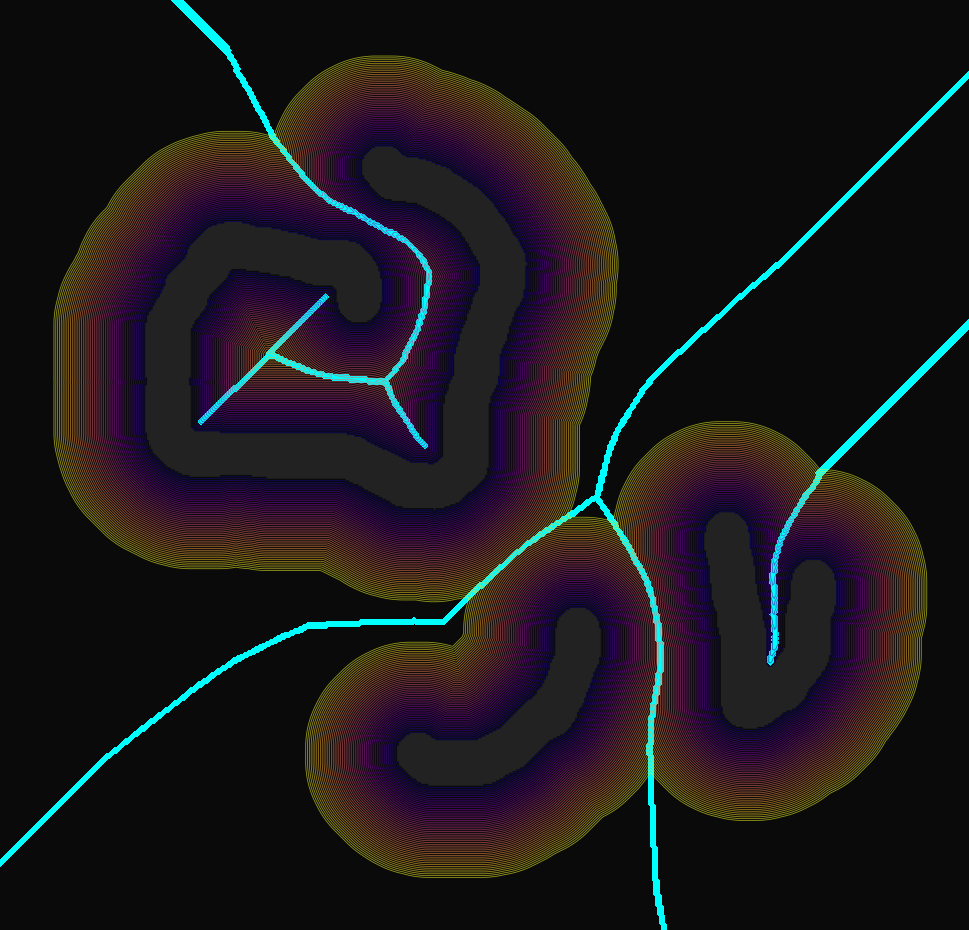
\includegraphics[width=\columnwidth]{infinitemedial.png}}
\caption{The raw medial axis skeleton (cyan) extracted directly from the SDF ridges. While the structure accurately captures the equidistant topological corridors between the local obstacles and isolated islands, it inherently generates unbounded external branches that extend infinitely into open space. Without geometric pruning, these protruding axes prevent the formation of a closed spatial manifold and cause gradient-based routing queries to diverge.}
\label{fig:raw_medial_axis}
\end{figure}


However, extracting $\mathcal{M}$ directly introduces a critical vulnerability: the \textit{Voronoi Void}. Because standard MAT algorithms strictly require equidistance between boundaries, expansive open spaces produce highly sparse, disconnected branches, or isolate topological "islands" representing free-standing obstacles. If the environment relies purely on $\mathcal{M}$, the global routing graph is fundamentally disconnected, stranding the robot in open space (see Appendix \ref{appendix:voronoi_void} for a visual and geometric elaboration of this failure mode).

\subsection{Geometric Bounding \& Internal Corridor Isolation}
Rather than deploying grid-search heuristics to bridge these voids, we utilize differential geometry to bound the structure. We first filter the raw medial axis to identify strictly internal, structured corridors. 

Let $\hat{t}_M(p)$ denote the unit tangent vector to the skeletal curve $\mathcal{M}$ at point $p$. Within a well-defined corridor, the medial axis runs parallel to the surrounding walls, meaning the SDF gradient $\nabla\Psi(p)$ points orthogonally to the curve. Let $\theta$ be the angle between the tangent $\hat{t}_M(p)$ and the gradient $\nabla\Psi(p)$. For a perfect corridor, $\theta = 90^\circ$. We evaluate the magnitude of the projection to isolate internal segments, defining the filtered subset $\mathcal{M}_{int}$ using an angular tolerance $\tau$ (e.g., $\tau = 17^\circ$):
\begin{equation}
    \mathcal{M}_{int} = \left\{ p \in \mathcal{M} \;\middle|\; \frac{|\hat{t}_M(p) \cdot \nabla\Psi(p)|}{\|\nabla\Psi(p)\|} \le \cos(90^\circ - \tau) \right\}
\end{equation}
As demonstrated in Fig. \ref{fig:angle_cutoff}, this condition successfully prunes infinitely protruding external branches (where $\theta$ diverges significantly) while isolating highly structured regions. Crucially, because the medial axis traversing the space between isolated islands also exhibits strong tangent-gradient parallelism, the identical $\theta \le 17^\circ$ threshold seamlessly preserves inter-island connectivity. This allows the algorithm to mathematically distinguish between bounded local topologies and unbounded external space, regardless of whether the obstacles form continuous walls or disjointed islands.

\begin{figure}[htbp]
\centerline{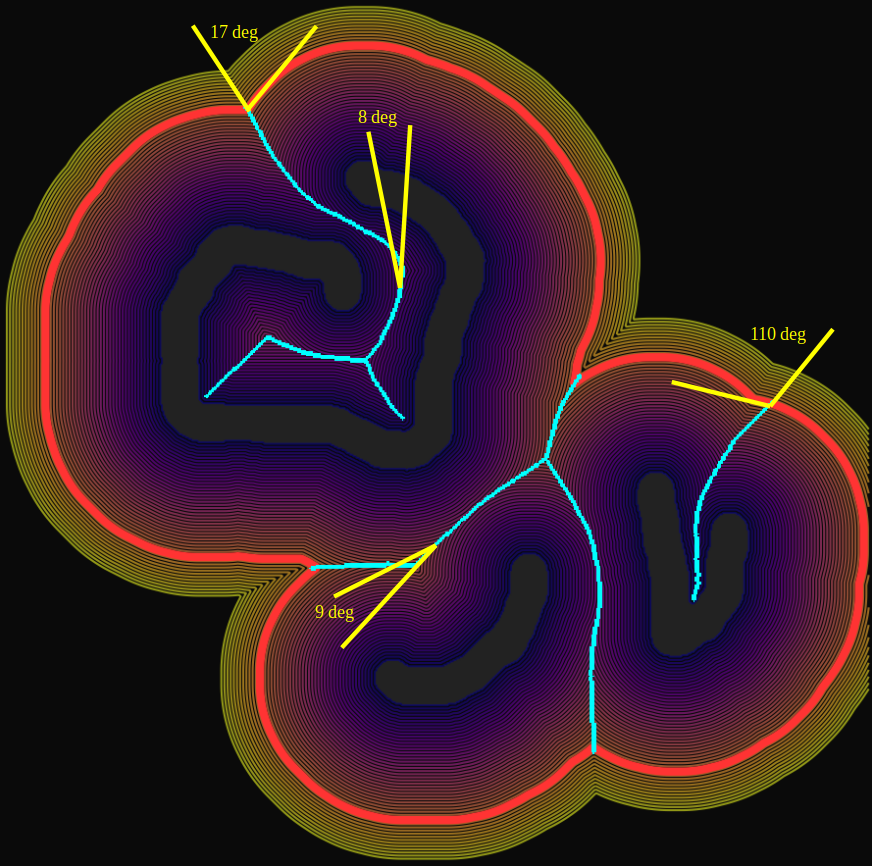
\includegraphics[width=\columnwidth]{angleprunning.png}}
\caption{Geometric bounding utilizing the tangent-gradient alignment condition across disjointed topologies. Enforcing an angular parallelism threshold ($\theta \le 17^\circ$) successfully identifies internal corridors (e.g., $8^\circ$) and prunes infinitely protruding external branches (e.g., $110^\circ$). Crucially, the medial axis formed between isolated obstacle islands also exhibits highly parallel SDF tangents (e.g., $9^\circ$). This allows the identical $17^\circ$ cutoff to seamlessly preserve inter-island connectivity. By applying a fixed offset (e.g., $\Delta_{offset} = 20$) to the maximum clearance of this preserved subset, a single continuous outer shell mathematically bounds the local interiors and isolated islands into one unified global cage.}
\label{fig:angle_cutoff}
\end{figure}


\subsection{Construction of the Topological Cage}
To permanently resolve the Voronoi Void and unify the graph, we construct a boundary that structurally encapsulates all isolated elements. Within the internal subset $\mathcal{M}_{int}$, we identify the absolute maximum clearance radius:
\begin{equation}
    C_{max} = \max_{p \in \mathcal{M}_{int}} \Psi(p)
\end{equation}
$C_{max}$ physically represents the radius of the widest bounded corridor in the environment. Using this scalar, we define a continuous outer bounding shell $\mathcal{B}_{outer}$ at a designated offset:
\begin{equation}
    d_{cage} = C_{max} + \Delta_{offset}
\end{equation}
\begin{equation}
    \mathcal{B}_{outer} = \{p \in \Omega \mid |\Psi(p) - d_{cage}| \le \epsilon \}
\end{equation}
The final \textit{Topological Cage}, denoted as $\mathcal{C}$, is mathematically defined as the union of the trimmed internal skeleton and this continuous outer shell:
\begin{equation}
    \mathcal{C} = \mathcal{M}_{trimmed} \cup \mathcal{B}_{outer}
\end{equation}
Because the outer shell $\mathcal{B}_{outer}$ is drawn at a distance strictly greater than any internal corridor radius (e.g., $ \Delta_{offset} = 20,$ yielding $d_{cage} > C_{max}$), it forms an inescapable closed topological envelope that mathematically bounds every smaller sub-region. Any isolated Voronoi islands, disconnected branches, or sparse voids residing within the open space are fully encapsulated by this bounding shell. Consequently, the once-fragmented spatial topology is united into a single, cohesive, bounded manifold ready for instantaneous $\mathcal{O}(1)$ query injections \textbf{(see Fig. \ref{fig:semantic_cage})}.


\begin{figure}[htbp]
\centerline{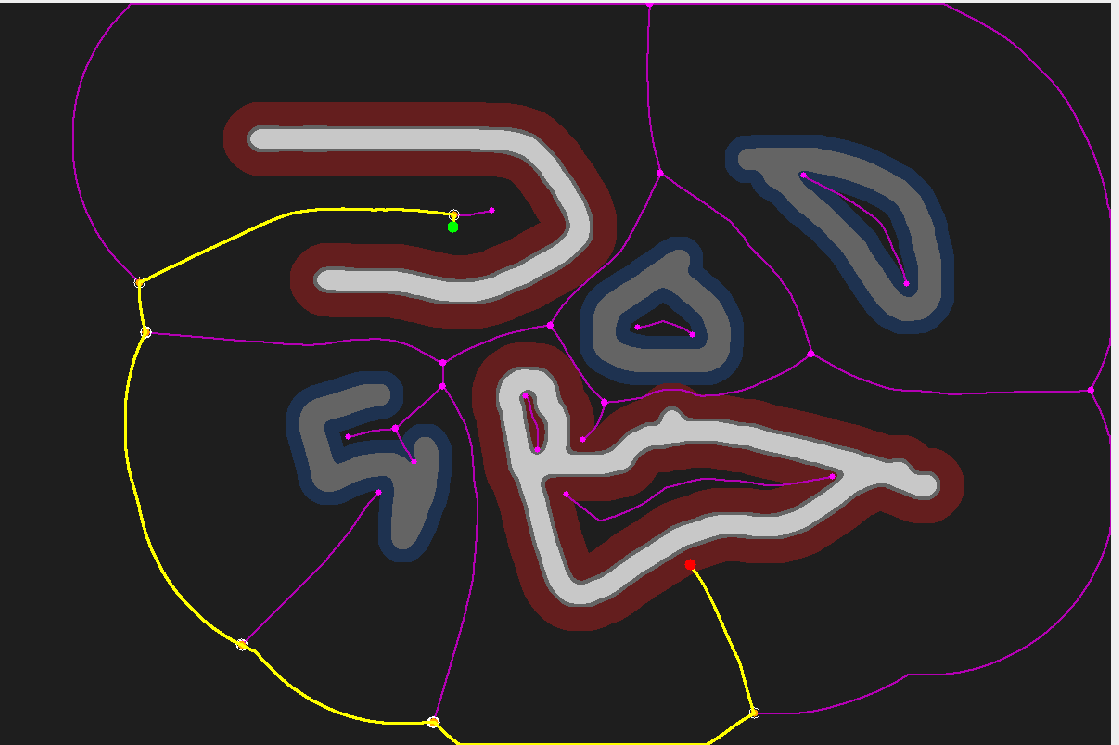
\includegraphics[width=\columnwidth]{medialplusband.png}}
\caption{Visualization of the fully constructed Topological Cage (purple) mapped over a semantically categorized environment. Obstacles are parameterized with distinct clearance thresholds, represented by visual bounding bands for rigid (red) and flexible (blue) constraints. The continuous outer offset shell seamlessly unifies all internal skeletal corridors and isolated structures into a single cohesive global graph, serving as the foundational manifold for subsequent routing queries (yellow).}
\label{fig:semantic_cage}
\end{figure}
% ==========================================
% V. METHODOLOGY PART 2: ONLINE PHASE
% ==========================================
\section{Methodology Part 2: Online Phase \& Mathematical Guarantees}
Once the Topological Cage $\mathcal{C}$ is constructed during the one-time offline phase, the system transitions to the online multi-query phase. By bypassing heuristic grid expansions, the algorithm routes arbitrary start ($p_S$) and goal ($p_G$) coordinates onto the cage in $\mathcal{O}(1)$ operations.

\subsection{Search-Less Gradient Injection}
To achieve search-less injection, we treat the arbitrary query points as particles subject to the continuous vector field $\nabla\Psi(x)$. From both $p_S$ and $p_G$, the algorithm deploys bi-directional ``scout'' trajectories that integrate along the normalized SDF gradient:
\begin{equation}
    p_{k+1} = p_k \pm \alpha \frac{\nabla\Psi(p_k)}{\|\nabla\Psi(p_k)\|}
\end{equation}
The positive integration ($+$) acts as a ``Climber'', aggressively ascending the spatial topography toward maximum clearance. Conversely, the negative integration ($-$) acts as a ``Diver''(Fig. \ref{fig:scouts}), descending toward the bounding shell. The integration immediately terminates upon intersecting any pixel belonging to $\mathcal{C}$.

\begin{figure}[htbp]
\centerline{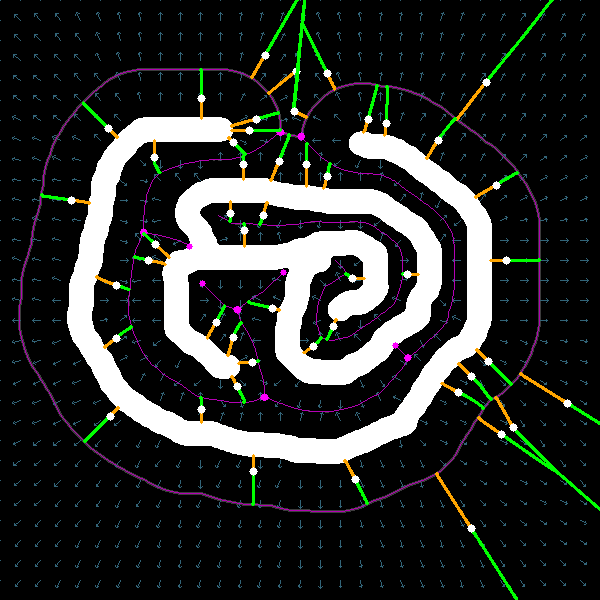
\includegraphics[width=0.8\columnwidth]{scout_navigation_map.png}}
\caption{Search-less start and goal injection via bi-directional gradient scouts. ``Climber'' (green) and ``Diver'' (orange) trajectories deterministically follow the local gradient vector field to intersect the overarching Topological Cage (purple). This provides visual proof of guaranteed finite-time graph connectivity from any arbitrary spatial coordinate without heuristic grid expansions.}
\label{fig:scouts}
\end{figure}

\subsection{Mathematical Guarantees of Convergence}
To strictly prove that grid-search can be permanently bypassed, we must mathematically guarantee that these continuous scouts will never enter infinite loops or wander endlessly.

\begin{theorem}[Topological Closure of the Bounding Shell]
Let $C_{max} = \max \Psi(p)$ for $p \in \mathcal{M}_{int}$. The boundary contour $L = \{p \in \Omega \mid \Psi(p) = C_{max} + \Delta_{offset}\}$ forms a strictly closed topological manifold that encapsulates all internal free-space structures, disconnected branches, and isolated Voronoi islands.
\end{theorem}
\begin{proof}
The Euclidean Signed Distance Function $\Psi(p)$ is globally Lipschitz continuous. The threshold $C_{max}$ represents the absolute supremum of obstacle clearance within the structured interior of the environment. By defining the limit $d_{cage} = C_{max} + \Delta_{offset}$, we guarantee that $d_{cage} > C_{max}$. Consequently, the level-set contour $L$ acts as a continuous bounding box encapsulating the internal structural geometry. Because $\mathcal{C}$ is defined as the union of the trimmed medial axis and this closed shell $L$, $\mathcal{C}$ itself constitutes a fully closed geometric set bounding the accessible free space.
\end{proof}

\begin{theorem}[Guaranteed Finite-Time Scout Convergence]
For any arbitrary starting coordinate $p_0 \in \Omega$, the monotonic gradient integration $\dot{p} = \pm \nabla\Psi(p)$ is guaranteed to intersect the Topological Cage $\mathcal{C}$ in finite distance.
\end{theorem}
\begin{proof}
The field $\Psi(p)$ possesses no local minima within the free space $\Omega$; local maxima exist strictly along the mathematical ridges of the Medial Axis $\mathcal{M}$. Integration along $\dot{p} = +\nabla\Psi(p)$ strictly and monotonically increases the scalar value of $\Psi(p)$. 

As the scout traverses $\Omega$, it is subject to only two geometric outcomes. First, it converges to a local maximum on the medial axis; because the internal medial axis is a subset of $\mathcal{C}$, it intersects $\mathcal{C}$. Second, if initialized in an expansive open void, it climbs away from obstacles until it crosses the boundary where $\Psi(p) = d_{cage}$. Because this closed contour $L$ is a fundamental subset of $\mathcal{C}$ (Theorem 1), it intersects $\mathcal{C}$. Due to the monotonic nature of the integration and the bounded environment, the streamline cannot oscillate. Therefore, intersection with $\mathcal{C}$ is deterministically guaranteed in finite length.
\end{proof}

\subsection{Discrete Graph Abstraction}
Because injection is mathematically guaranteed without grid search, the continuous spatial problem collapses into a highly sparse, discrete graph $G = (V, E)$. The vertices $V$ consist solely of the critical junction nodes of $\mathcal{C}$ and the injected connection points $p_S'$ and $p_G'$. Crucially, this discrete abstraction inherently supports dynamic environment updates; in the presence of localized obstacle movement, the affected subset of graph edges can be rapidly pruned and locally re-routed without triggering a full global reconstruction of the Topological Cage. Graph routing using Yen's K-Shortest Paths algorithm occurs instantaneously, rendering the global pathfinding complexity effectively $\mathcal{O}(1)$ with respect to total map area.

% ==========================================
% VI. METHODOLOGY PART 3: PHYSICS OPTIMIZATION
% ==========================================
\section{Methodology Part 3: Exhaustive Path Sampling \& Physics Optimization}
While the topological route guarantees clearance, skeletonized paths are inherently safest but un-optimized. To execute smooth kinematics on physical hardware, we aggressively optimize the trajectory through exhaustive sampling and a dynamic physics tensioner.

\subsection{Lexicographical Bottleneck Evaluator}
As illustrated in Fig. \ref{fig:lexicographical}, the extreme computational efficiency of the $\mathcal{O}(1)$ injection affords the system a massive time budget. Rather than settling for a single heuristic route, the algorithm exhaustively evaluates all topological combinations generated from both the ``Climber'' and ``Diver'' scouts. 

To select the absolute safest homotopy class among $K$ distinct paths, we introduce a Lexicographical Bottleneck Evaluator. For each extracted path, the SDF values of all traversed pixels are compiled and sorted in ascending order. The algorithm compares these sorted arrays as decimal values. This mathematically guarantees that the planner selects the path with the widest minimum bottleneck constraint, flawlessly resolving ties when multiple paths share a common tight starting corridor.

\begin{figure*}[htbp] % Using figure* to span both columns if the image is wide
\centerline{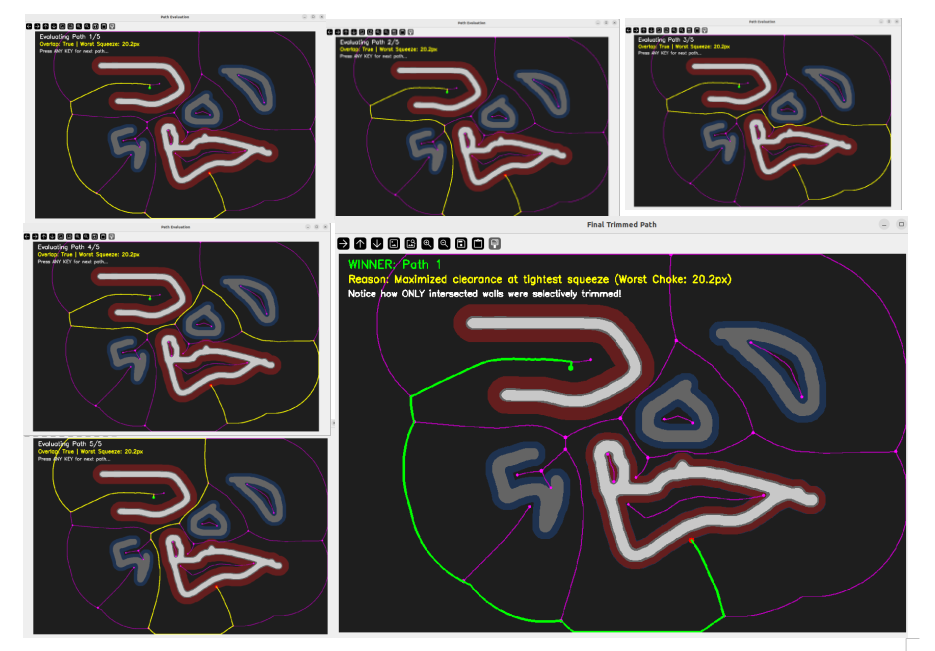
\includegraphics[width=\textwidth]{safepathcomparisions.png}}
\caption{Real-time exhaustive homotopy evaluation. Utilizing the ultra-fast $\mathcal{O}(1)$ injection, the planner extracts $K$ distinct macroscopic paths and applies a Lexicographical Bottleneck Evaluator. By sorting the SDF values of each route, the algorithm deterministically selects the optimal path (bottom right) that maximizes structural clearance at the environment's most constrained choke point.}
\label{fig:lexicographical}
\end{figure*}

\subsection{Selective Adaptive Trimming}
Standard elastic band planners frequently fail because rigid obstacle repulsion fields overpower the path tension in narrow corridors, causing the robot to freeze. We resolve this by applying Selective Adaptive Trimming to the optimal path. 

The algorithm assigns unique integer IDs to every disconnected obstacle via a connected components analysis. It then scans the chosen path to find the absolute tightest squeeze for each specific obstacle ID it intersects. The SDF repulsion threshold is dynamically lowered \textit{only} for those specific intersected walls, creating a custom shrink-wrapped constraint that allows the elastic band to pass without violent repulsion. 

\subsection{True Spring-Mass Tensioning \& Auto-Stabilization}
The final jagged path is smoothed using a True Spring-Mass elastic band. We discretize the trajectory into movable nodes $P_i$. Unlike basic elastic bands that suffer from node clumping, we enforce a strict resting length using Hooke's Law alongside kinetic damping. The acceleration of each node is governed by:
\begin{equation}
    \ddot{P}_i = W_{s} \vec{F}_{spring} + W_{r} \vec{F}_{repel} - D\dot{P}_i
\end{equation}
where $W_{s}$ and $W_{r}$ are tuning weights, $D$ is the kinetic damping (friction) coefficient, and the forces are defined as:
\begin{equation}
    \vec{F}_{spring} = \sum_{j \in \{i-1, i+1\}} \left( \frac{P_j - P_i}{\|P_j - P_i\|} \right) \big( \|P_j - P_i\| - d_{rest} \big)
\end{equation}
\begin{equation}
    \vec{F}_{repel} = \sum_{O \in \{Rigid, Soft\}} \left( \frac{\nabla\Psi_O(P_i)}{\|\nabla\Psi_O(P_i)\|} \right) \big( \tau_O - \Psi_O(P_i) \big)
\end{equation}
where $d_{rest}$ is the ideal structural spacing, and $\tau_O$ represents the selectively trimmed repulsion limits for rigid and soft walls.

To physically tighten the rope around corners, we utilize \textit{Distributed Popping}. Rather than aggressively deleting nodes at the edges, the algorithm periodically deletes every $N$-th node uniformly across the entire length of the rope. This ensures massive slack loops are pulled tight simultaneously. 

Because kinetic damping absorbs the bouncy kinetic energy, the nodes gracefully slide against the trimmed walls and lose momentum. The system continuously tracks the maximum movement velocity of all nodes. Once the maximum velocity drops below a stability threshold $\epsilon_{stable}$ for a set duration of frames, the system autonomously triggers an Auto-Stop, guaranteeing a perfectly optimized and settled trajectory ready for robotic execution. (Fig. \ref{fig:rope_tensioner})

\begin{figure}[htbp]
\centerline{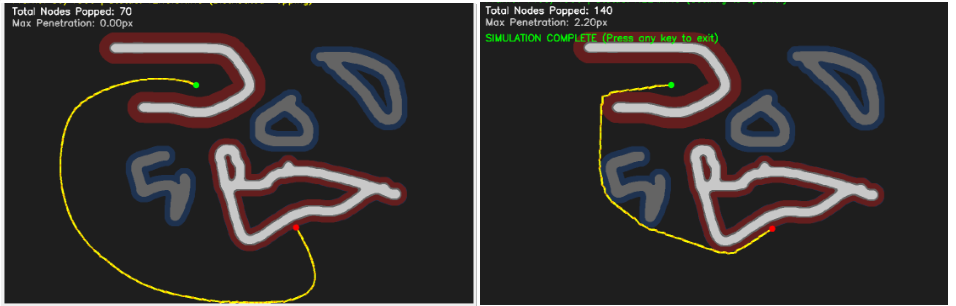
\includegraphics[width=1.0\columnwidth]{compiled image of the rope tensioner routine.png}}
\caption{Kinematic optimization via the True Spring-Mass tensioner. The un-optimized, jagged topological safe path derived from the lexicographical evaluator (left) is dynamically smoothed (right) using distributed node popping and kinetic damping. The optimized trajectory rests precisely against selectively trimmed SDF thresholds, yielding an executable path free of local-minima oscillations.}
\label{fig:rope_tensioner}
\end{figure}

% ==========================================
% VII. EXPERIMENTAL SETUP
% ==========================================
\section{Experimental Setup}
To validate the theoretical guarantees of the Topological Cage within real-world dynamic constraints, we deployed the proposed algorithm on a physical robotic testbed. 

\textbf{A. Hardware and Projection Architecture} \\
The physical experiments were conducted using a differential-drive TurtleBot 3 platform. To seamlessly fuse the algorithmic abstraction with the physical environment, we utilized a MacCap (motion-capture) system equipped with high-lumen overhead projectors. The binary occupancy map, the computed Topological Cage, the bi-directional gradient scouts, and the real-time true spring-mass elastic band were projected directly onto the laboratory floor. This provided immediate, visual, one-to-one correspondence between the mathematical physics engine and the physical space.

\textbf{B. Control and ROS Integration} \\
The spatial state of the TurtleBot was continuously tracked via roof-mounted cameras identifying an ArUco marker array on the robot's chassis. This pose data was streamed to a central processing node and broadcast to the ROS \texttt{tf} (transform) tree. 

The Topological Cage algorithm handled global routing entirely offline. Upon receiving an arbitrary goal query, the algorithm performed the $\mathcal{O}(1)$ gradient injection, lexicographical tie-breaking, and adaptive physics tensioning. The resulting smoothed coordinates were published as a dense \texttt{nav\_msgs/Path} to a standard Pure Pursuit local controller, which computed the necessary velocity commands (\texttt{cmd\_vel}) to physically drive the TurtleBot along the tensioned elastic band.

% ==========================================
% VIII. RESULTS & BENCHMARKS
% ==========================================
\section{Results \& Benchmarks}
We benchmarked the Topological Cage framework against standard planners available in the ROS Navigation Stack: the Timed Elastic Band (TEB) local planner, the Dynamic Window Approach (DWA), A*, and Probabilistic Roadmaps (PRM).

\subsection{Multi-Query Computational Amortization}
The primary vulnerability of standard grid-search algorithms is their linear scaling with respect to the number of queries. We tasked the planners with resolving 100 consecutive random start-to-goal queries in a dense, highly constrained map. 

As detailed in Table \ref{tab:compute_benchmarks}, A* required a full grid expansion for every individual query, resulting in cumulative processing times exceeding 300 seconds. While PRM is natively designed for multi-query scenarios, its random sampling required a dense node distribution to capture narrow doorways, bloating its query evaluation time.

In contrast, our proposed SDF-Derived Topological Skeletonization (SDTS) framework paid a one-time offline preprocessing cost of approximately $189$ ms to construct the continuous SDF and the Topological Cage. Subsequent online queries, driven strictly by the search-less gradient injection and sparse topological routing, averaged less than $30$ ms per route. For multi-agent systems or complex waypoint sequences, this $\mathcal{O}(1)$ decoupling represents an overwhelming computational dominance.

\begin{table}[htbp]
\caption{Computational Efficiency in Multi-Query Scenarios}
\begin{center}
\begin{tabular}{@{}lccc@{}}
\toprule
\textbf{Algorithm} & \textbf{Offline Prep (ms)} & \textbf{Avg Query (ms)} & \textbf{Total for 100 (s)} \\ \midrule
A* & 0.0 & $3695.9$ & $369.6$ \\
PRM (Dense) & $430.7$ & $41.2$ & $4.55$ \\
\textbf{SDTS (Ours)} & $\textbf{189.2}$ & $\textbf{28.3}$ & $\textbf{3.02}$ \\ \bottomrule
\end{tabular}
\label{tab:compute_benchmarks}
\end{center}
\end{table}

\subsection{Voronoi Void and Trap Resolution}
We evaluated the algorithms in adversarial geometric topologies: massive open spaces causing the "Voronoi Void", and tightly confined U-shaped non-convex traps. 

In expansive open rooms, standard skeletonization planners generated sparse, disconnected branches, leaving query points stranded and unable to connect to the graph. As illustrated in Appendix \ref{appendix:voronoi_void},and Fig. \ref{fig:isolated_island}, our Topological Cage utilized the bounding shell to mathematically envelop these islands, ensuring the bi-directional scouts deterministically intersected the unified global graph without resorting to heuristic flood-fills.

In U-shaped traps, DWA frequently collapsed into local minima, while RRT* consistently failed to navigate the narrow exit corridors. While TEB successfully navigated the topology, its rigid obstacle repulsion penalties resulted in violent oscillatory behavior when passing through tight doors. The Topological Cage resolved these traps flawlessly: the lexicographical evaluator guaranteed the widest available homotopy class, and the Selective Adaptive Trimming seamlessly shrink-wrapped the SDF constraints at the bottleneck, allowing the elastic band to pass without triggering severe repulsion forces.

\begin{figure}[htbp]
\centerline{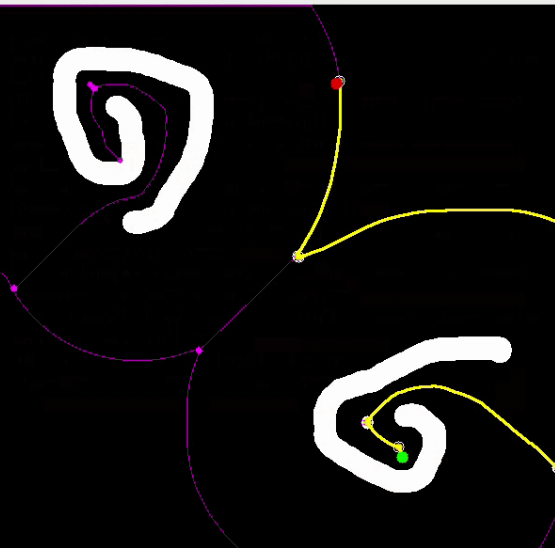
\includegraphics[width=0.8\columnwidth]{isolated_island_navigation.png}}
\caption{Proof of concept for the Voronoi Void resolution. The algorithm mathematically unites geometrically disjointed, isolated obstacle islands via the continuous offset shell (purple). Bi-directional off-graph queries successfully route into the unified skeleton, proving the framework's robustness in expansive open spaces devoid of standard Voronoi corridors.}
\label{fig:isolated_island}
\end{figure}

\subsection{Trajectory Kinematics and Smoothness}
While medial axis paths natively maximize clearance, they are characterized by sharp, jagged corners unsuitable for smooth differential-drive execution. We evaluated the physical odometry of the TurtleBot traversing both the raw skeletonized path and the path optimized by our True Spring-Mass tensioner.

The introduction of strict Hooke's Law resting lengths combined with kinetic damping effectively eliminated the node-clumping phenomena observed in basic elastic bands. Furthermore, the distributed node popping ensured that slack loops were pulled tight symmetrically. The physical execution tracking demonstrated a massive reduction in trajectory curvature and angular jerk. Because the kinetic energy tracker autonomously terminated the physics engine precisely when the system stabilized, the robot was fed an optimally smooth, highly safe path entirely devoid of narrow-corridor oscillations.

% ==========================================
% IX. CONCLUSION
% ==========================================
\section{Conclusion}
This paper presented the Topological Cage, a search-less geometric framework that bridges the critical gap between global skeletonization and local elastic band optimization. By modeling free space as a continuous vector field, we successfully bounded the medial axis, permanently resolving the injection problem and eliminating disjointed Voronoi Voids. 

By front-loading grid computations into a single offline abstraction, the algorithm achieves lightning-fast, $\mathcal{O}(1)$ online multi-query routing. This extreme computational efficiency allows for the exhaustive sampling and lexicographical evaluation of multiple homotopy classes in real time. Finally, the combination of selective adaptive SDF trimming and a distributed spring-mass physics engine yields an optimally smooth, provably safe trajectory. Real-world validation on physical hardware demonstrates that structural differential geometry, when bounded and evaluated deterministically, provides an incredibly robust and computationally superior alternative to exhaustive graph-search and purely heuristic navigation paradigms. Furthermore, the extreme sparsity of the Topological Cage establishes a foundation for dynamic adaptability, where localized obstacle movements can be accommodated through targeted graph pruning rather than global recalculations—an avenue we intend to explore in future work.


% ==========================================
% APPENDIX
% ==========================================
\appendices
\section{Addressing the Voronoi Void and Injection Problem}
\label{appendix:voronoi_void}

A critical failure point in standard topological planners occurs in massive open spaces, a phenomenon we term the ``Voronoi Void'' (see Fig. \ref{fig:voronoi_problem}). Standard Voronoi generation relies on points being strictly equidistant between two or more obstacle boundaries. In expansive open rooms, the traditional Voronoi skeleton often fails by generating sparse, disconnected branches or leaving massive dead zones entirely devoid of a navigational highway.

\begin{figure}[htbp]
\centerline{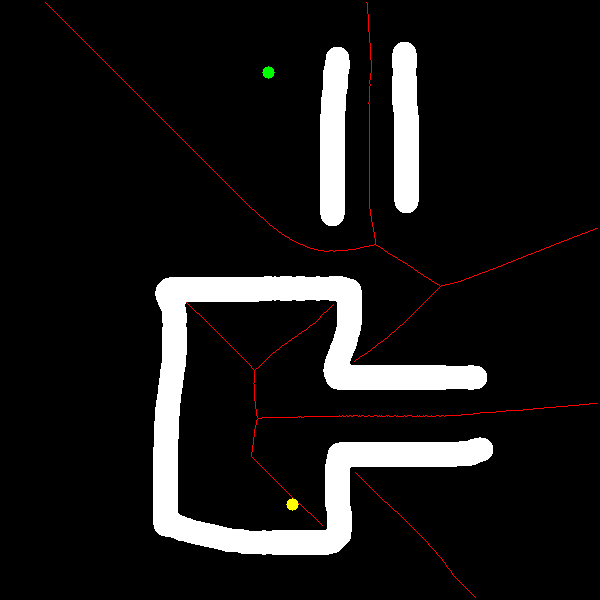
\includegraphics[width=0.8\columnwidth]{voronoi_shortcoming_raw.png}}
\caption{The Voronoi Void trap. The standard Voronoi medial axis (red lines) relies strictly on equidistance, providing zero structural guidance in the expansive open space and stranding the arbitrary query point (green dot).}
\label{fig:voronoi_problem}
\end{figure}

If a robot is initialized deep within such a void, traditional planners are forced to fall back on heuristic grid searches like A* or Breadth-First Search (BFS) simply to reach the nearest graph node, requiring the discretization of the entire open space.

The proposed SDF-Derived Topological Skeletonization (SDTS) framework entirely bypasses this expensive flood-fill operation. Rather than relying solely on the static skeletal graph, our method exploits the continuous underlying vector field of the entire free space to encapsulate the environment.

\begin{figure}[htbp]
\centerline{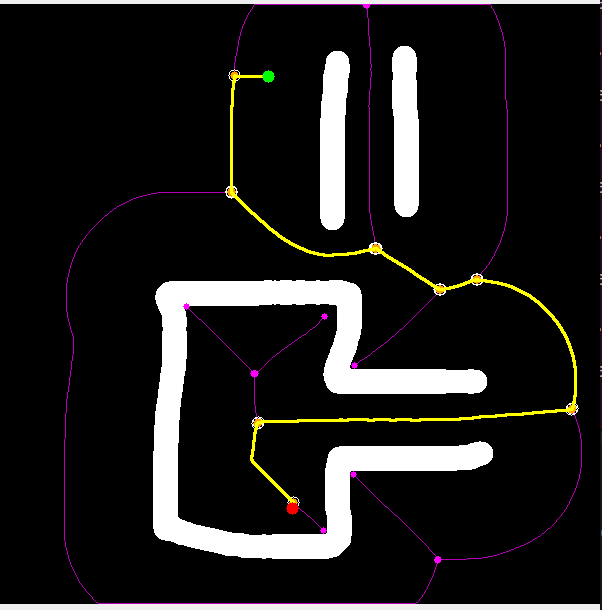
\includegraphics[width=0.8\columnwidth]{voronoi_our_path.png}}
\caption{Resolution via the Topological Cage (purple boundary). Gradient-driven scouts deterministically route arbitrary off-road query points to the unified skeletal network (yellow path) without requiring any heuristic grid expansions.}
\label{fig:voronoi_resolution}
\end{figure}

As shown in Fig. \ref{fig:voronoi_resolution}, by evaluating the omnipresent field $\Psi(x)$ continuously, the ``Climber'' scout deterministically steps along the gradient vector, mathematically ascending the clearance topology. Because the skeletal highway is encapsulated within the closed Topological Cage $\mathcal{C}$, this gradient ascent is geometrically guaranteed to intersect the cage in finite time, requiring only $\mathcal{O}(1)$ operations per step and effortlessly linking isolated coordinates to the global routing network.s
% ==========================================
% REFERENCES
% ==========================================
\begin{thebibliography}{00}
\bibitem{teb} C. Rösmann, W. Feiten, T. Wösch, F. Hoffmann and T. Bertram, "Trajectory modification considering dynamic constraints of autonomous robots," \textit{7th German Conference on Robotics (ROBOTIK)}, Munich, 2012, pp. 1-6.
\bibitem{dwa} D. Fox, W. Burgard, and S. Thrun, "The dynamic window approach to collision avoidance," \textit{IEEE Robotics \& Automation Magazine}, vol. 4, no. 1, pp. 23-33, 1997.
\bibitem{edt} P. F. Felzenszwalb and D. P. Huttenlocher, "Distance transforms of sampled functions," \textit{Theory of Computing}, vol. 8, no. 1, pp. 415-428, 2012.
\bibitem{rrt} S. M. LaValle, "Rapidly-exploring random trees: A new tool for path planning," TR 98-11, Computer Science Department, Iowa State University, 1998.
\bibitem{prm} L. E. Kavraki, P. Svestka, J. -C. Latombe and M. H. Overmars, "Probabilistic roadmaps for path planning in high-dimensional configuration spaces," \textit{IEEE Transactions on Robotics and Automation}, vol. 12, no. 4, pp. 566-580, 1996.
\end{thebibliography}

\end{document}

\end{document}